
\begin{figure}[h!]
    \centering
    \resizebox{0.45\textwidth}{!}{
        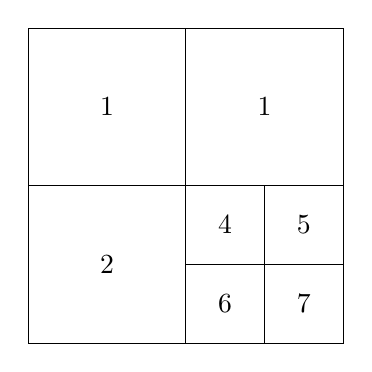
\begin{tikzpicture}
            \draw (1, 1) rectangle (3, 3);
            \node at (2, 2){2};
            \draw (1,3) rectangle (3, 5);
            \node at (2, 4) {1};
            \draw (3, 3) rectangle (5, 5);
            \node at (4, 4) {1};
            \draw (3, 1) rectangle (4, 2);
            \node at (3.5, 1.5) {6};
            \draw (3, 2) rectangle (4, 3);
            \node at (3.5, 2.5) {4};
            \draw (4, 1) rectangle (5, 2);
            \node at (4.5, 1.5) {7};
            \draw (4, 2) rectangle (5, 3);
            \node at (4.5, 2.5) {5};
        \end{tikzpicture}
    }
    \caption{Квадратная матрица, разделенная на квадранты}
    \label{qmatrix}
\end{figure}
\begin{figure}[h!]
    \centering
    \Tree [.A
            [.{Leaf(1, 2)}  ]
            [.{Leaf(1, 2)}  ]
            [.{Leaf(2, 2)}  ]
            [.SE
                    [.{Leaf(4, 1)}  ]
                    [.{Leaf(5, 1)}  ]
                    [.{Leaf(6, 1)}  ]
                    [.{Leaf(7, 1)}  ]
            ]
        !\qsetw{0.5cm}
    ]
    \caption{Изображение дерева квадрантов в виде дерева}
    \label{qtree1}
\end{figure}
